\documentclass[11pt]{article}

\usepackage{graphicx}

% Enable references to labels in the notes
\usepackage{xr-hyper}
\externaldocument{p328_notes}
\usepackage{hyperref}

% Sans fonts
\usepackage{sfmath}
\renewcommand{\familydefault}{\sfdefault}

\newcommand{\COURSE}{PHYS328W}
\newcommand{\LABNUM}{2}
\newcommand{\TITLE}{Kirchhoff's Rules and Equivalent Circuits}
\markright{\COURSE~Lab \LABNUM\ : \TITLE}

\setlength{\textwidth} {6.5 true in}
\setlength{\textheight}{9 true in}
\setlength{\hoffset}   {-0.75 true in}
\setlength{\voffset}   {-0.75 true in}
\setlength{\parindent} {12 pt}
\pagestyle{myheadings}

\begin{document}

\thispagestyle{empty}

\section*{\COURSE\ Lab \LABNUM\ : \TITLE}

This assignment relies on Sections~\ref{sec:kirchhoff} and
\ref{sec:thevenin} of the notes.

\subsection*{Experiments}

\begin{figure}[h]
  \centering
  \scalebox{1.0}{
    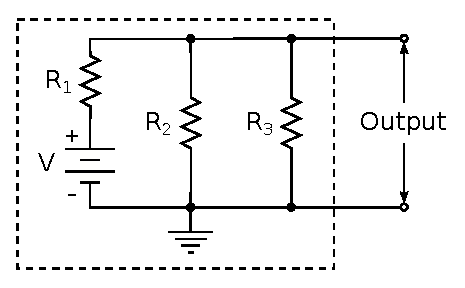
\includegraphics{thevenincircuit.eps}
  }
  \caption{Schematic of the circuit for testing Kirchoff's rules and
    Th\'{e}venin analysis.} 
  \label{fig:thevenincircuit}
\end{figure}

\begin{enumerate}
\item Find three different resistors in the 1-10~k$\Omega$ range, and
  a 1~k$\Omega$ resistor to use as a load in
  step~\ref{step:thevenin}. Measure their resistances with a DMM.

\item Construct the circuit shown in
  Figure~\ref{fig:thevenincircuit}. Use the 5~V power supply on the
  prototyping board.

\item Use a DMM to measure the supply voltage and the voltage drops
  across the three resistors. Check that your measured voltage drops
  make sense (i.e. satisfy the loop rule).

\item Use the measured resistances and voltage drops to determine all
  of the unique currents flowing in the circuit. Check that these
  currents make sense (i.e. satisfy the junction rule).

\item Sketch the circuit in your log book, and label the currents with
  arrows. \textit{To get the directions, if the DMM shows a positive
  voltage reading across a resistor, current is flowing from the
  point connected to the red lead (V$\Omega$) to the point connected
  to the black lead (COM) of the DMM. Current flows ``down hill'' in
  the potential landscape.}

\item \label{step:thevenin} Add the 1~k$\Omega$ load resistor to the
  circuit, and measure its voltage drop and the current flowing
  through it.
\end{enumerate}

\subsection*{Calculations}

In your log book ...

\begin{enumerate}
\item Use Kirchhoff's rules to calculate the currents flowing in the
  circuit shown in Figure~\ref{fig:thevenincircuit} with no load
  resistor, assuming your measured resistances and supply
  voltage. Then calculate the open-circuit output voltage.

\item Calculate the Th\'{e}venin voltage $V_{th}$ and resistance
  $R_{th}$ of your circuit, treating the voltage across $R_3$ as the
  output as illustrated by Figure~\ref{fig:thevenincircuit}.

\item Use $V_{th}$ and $R_{th}$ to predict the current through and
  the voltage across a 1~k$\Omega$ load resistor driven by your
  circuit.
\end{enumerate}

\subsection*{Simulations}

We will be using \texttt{OrCAD Capture Lite} to design and simulate
circuits throughout the course. A brief guide is included in
Appendix~\ref{sec:orcad} of the notes. We will work on simulating this
first circuit together in class --- be sure to take notes in your log
book on how to use the software. 
\begin{enumerate}
  \item Simulate the circuit with no load.
    \begin{itemize}
    \item Start a new, blank project in \texttt{OrCAD Capture Lite}, and
      build your resistor network circuit.

    \item Use the 
\includegraphics{OrCAD_NewSimProf.png} (or
      \texttt{PSpice->New Simulation Profile}) to create a
      \texttt{Transient (Time Domain)} analysis profile. 
      \emph{The default settings are fine in this case, since there is
        no time dependence in the behavior of this circuit.}

    \item Click on the 
\includegraphics{OrCAD_RunSim.png} button in the
      tool bar to run the PSpice simulation. 
      
    \item Click on the 
\includegraphics{OrCAD_ShowV.png} and
      
\includegraphics{OrCAD_ShowI.png} buttons in the tool bar
      to show the values from the simulation in the schematic window, and
      compare them with your measurements and calculations.
    \end{itemize}

  \item Make a new simulation of your circuit driving a 1~k$\Omega$
    load resistor. Compare the current through and voltage across the
    load resistor with your theoretical prediction.

  \item Make a new simulation of the Th\'{e}venin equivalent circuit
    driving a 1~k$\Omega$ load.
\end{enumerate}

\subsection*{Products}

Upload to Canvas the PDF of a brief \LaTeX\ report in which you ...
\begin{itemize}
\item  Discuss the degree of agreement between your measurements,
  theoretical predictions, and simulations.

\item Comment on the degree to which your observations align with
  Th\'{e}venin's theorem.

\item Include as figures ...
  \begin{itemize}
  \item A scan or image of the labeled schematic of your resistor
    newtork circuit from your log book.

  \item Screen shots of the schematics of your three simulations
    showing simulated voltages and currents.

  \item A scan or image of your Kirchhoff's-rules and
    Th\'{e}venin-equivalent-circuit calculations from your log book.
  \end{itemize}
\end{itemize}

\end{document}
